%\externaldocument{./../tex/MAVBench.tex}

\section{Closed-loop Simulation}
\label{sec:simulation}
\setstcolor{red}

We discuss a closed-loop simulation environment for simulating and studying MAVs. In \Sec{sec:components}, we describe the components of a MAV, how they interact and why the intra- and inter-system interactions are important to capture. In \Sec{sec:setup}, we show how our setup captures these components and their interactions in a closed-loop setup. In \Sec{sec:energy}, we describe how the simulator models energy consumption, in addition to the functional and performance data described in the earlier section. In \Sec{sec:knobs}, we describe the knobs that our simulator supports to enable exploratory studies, and in \Sec{sec:accuracy}, we describe the limitations of our current setup and opportunities for future enhancements. 
 
\begin{figure}[t!]
\centering
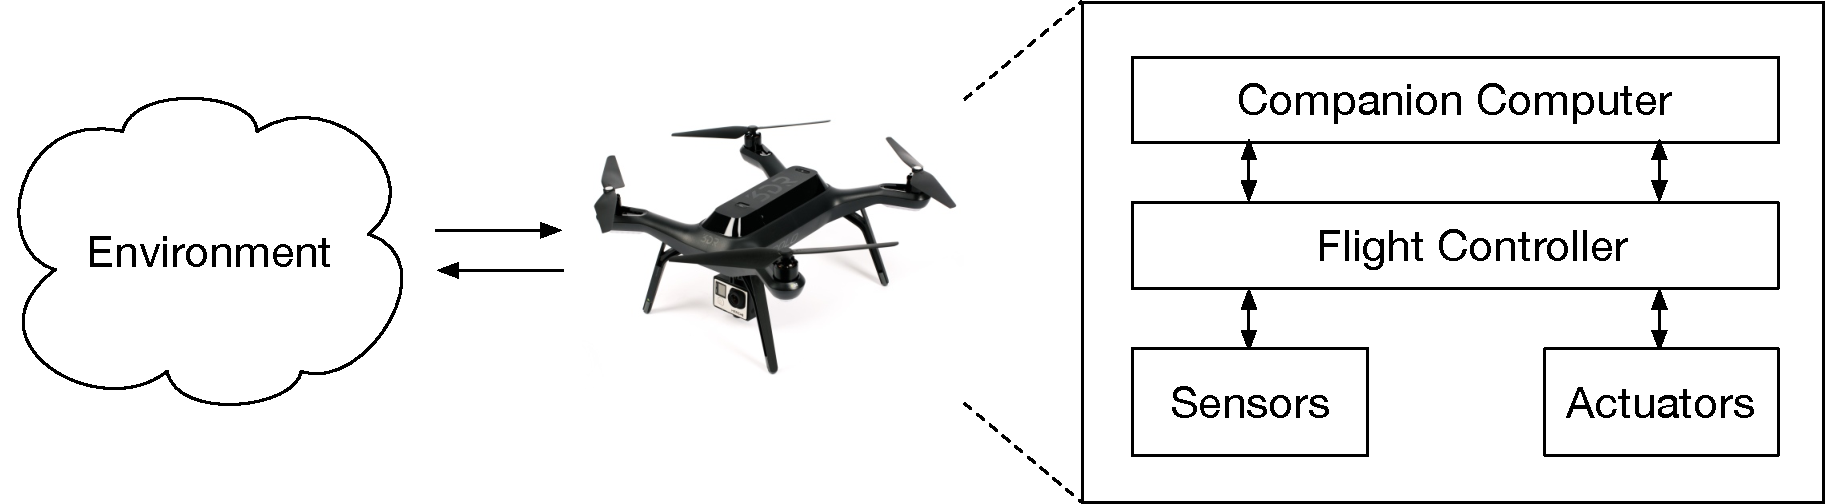
\includegraphics[trim=0 0 0 -25, clip, width=0.9\linewidth]{figs/Aerial_agent_3}
\caption{Closed-loop data flow in a MAV. Information flows from sensors collecting environment data into the MAV's compute system, down into the actuators and back to the environment.}
\label{fig:Aerial_agent_data_flow}
\end{figure}

\subsection{MAV System Components Dissected}
\label{sec:components}

Closed-loop operation is an integral component of autonomous MAVs. In such systems, the data flows in a (closed) loop, starting from the environment, going through the MAV and back to the environment as shown in \Fig{fig:Aerial_agent_data_flow}. The process involves sensing the environment (Sensors), interpreting it and making decisions (Compute), and finally navigating within or modifying the environment (Actuators) in a loop. 

\paragraph{Sensors:} Sensors are responsible for capturing the state associated with the agent and its surrounding environment. 
To enable intelligent flights, MAVs must be equipped with a rich set of sensors capable of gathering various forms of data such as depth, position, and orientation. For example, \mbox{RGB-D} cameras can be utilized for determining obstacle distances and positions. The number and the type of sensors are highly dependent on the workload requirements and the compute capability of on board processors for their interpretations.


%\textbf{Perception/Control:} A flight controller and a companion computer provide the compute power for high-level and low-level functions such as object detection and rotor controls. 
\paragraph{Flight Controller (Compute):} The flight controller (FC) is an autopilot system responsible for the MAV's stabilization and conversion of high-level to low-level actuation commands. 
While they themselves come with basic sensors, such as gyroscopes and accelerometers, they are also used as a hub for incoming data from other sensors such as GPS, sonar, etc. For command conversions, FCs take high-level flight commands such as``take-off" and lower them to a series of instructions understandable by actuators such as rotors. FCs use light-weight processors such as the ARM Cortex-M3 32-bit RISC core for the aforementioned tasks.    
 
\paragraph{Companion Computer (Compute):} The companion computer is a powerful compute unit (compared to the FC) that is responsible for the processing of the high level, computationally intensive tasks such as vision processing. Not all MAVs come equipped with companion computers, rather these are typically an add-on option for more processing. NVIDIA's TX2 is a representative example with significantly more compute capability than an FC.

{\paragraph{Actuators:} Actuators allow agents to react to their surroundings and further modify them. They range anywhere from rather simple rotors to robotic arms capable of grasping and lifting objects. Similar to sensors, their type and number is a function of the workload and processing power on board.

\begin{comment}
\subsection{Simulator requirements}
As the system architecture in section III reveals, data flows in a loop for robotic applications, i.e. starting from environment and its sensing to perception, from perception to actuation and back to the environment where its ready to be sensed again. Aerial computing architectural analysis/synthesis demands fast end-to-end simulator, capable of mimicking this closed-loop flow and capturing the interactions across layers. In this section 
%, such features ensure problem identification and solution verification feasibility, and hence allowing simulators to fulfill their role (refer to the other paper).
we discuss how absence/presence of these conditions have architectural ripples. Since simulator design is a never ending battle between accuracy and speed, we analyze the space using these two lenses.


\textit{system/env interactions (Accuracy Impact):} Lacking end-to-end simulation capabilities deprives researcher of design opportunities system/environment interaction consideration provides. In addition, forgoing these interactions can also lead to bottleneck misidentification ,and hence over optimizations. 

(possibly studying the affect of obstacle density on motion planning processing time (and frequency) and deciding whether an accelerator is necessary or not (depending on the env)

\textit{Intra system interactions (Accuracy Impact):} 
Lacking end-to-end inspection can mean having to study application kernels in isolation and hence overlooking the necessary analysis of inter kernels interactions and a design synthesis around it.
examples: 
(1)running slam and object detection and slower than both. But, we gpu zero sharing (for images), we might be able to improve performance.
(2) impact of having bigger caches on delivery last phase (when detection is running. We might be able to model this by lowering the octomap resolution so it'll take less space in the caches)
(3) cache pollution, branch prediction interference.  
//the example need to be 
environment independent, but rather application dependent
   
\textit{speed Impact:}
Wanting to capture above interactions, and given the long mission times (throw some numbers) and irregularity of the environment causing application phases changes, fast simulators are necessary. pure cycle accurate simulators are inviable since it takes ... time to .... 

We believe that a hybrid solution where real embedded-systems, placed in the loop (HIL style) for bottle-neck identification, augmented with an fpga or cycle accurate simulator for testing new ideas is winner solution. 
\end{comment}


\subsection{Simulation Setup}
\label{sec:setup}

We present how our setup, shown in \Fig{fig:end-to-end}, maps to the various components corresponding to a MAV's operation.

\begin{figure}[t!]
\centering
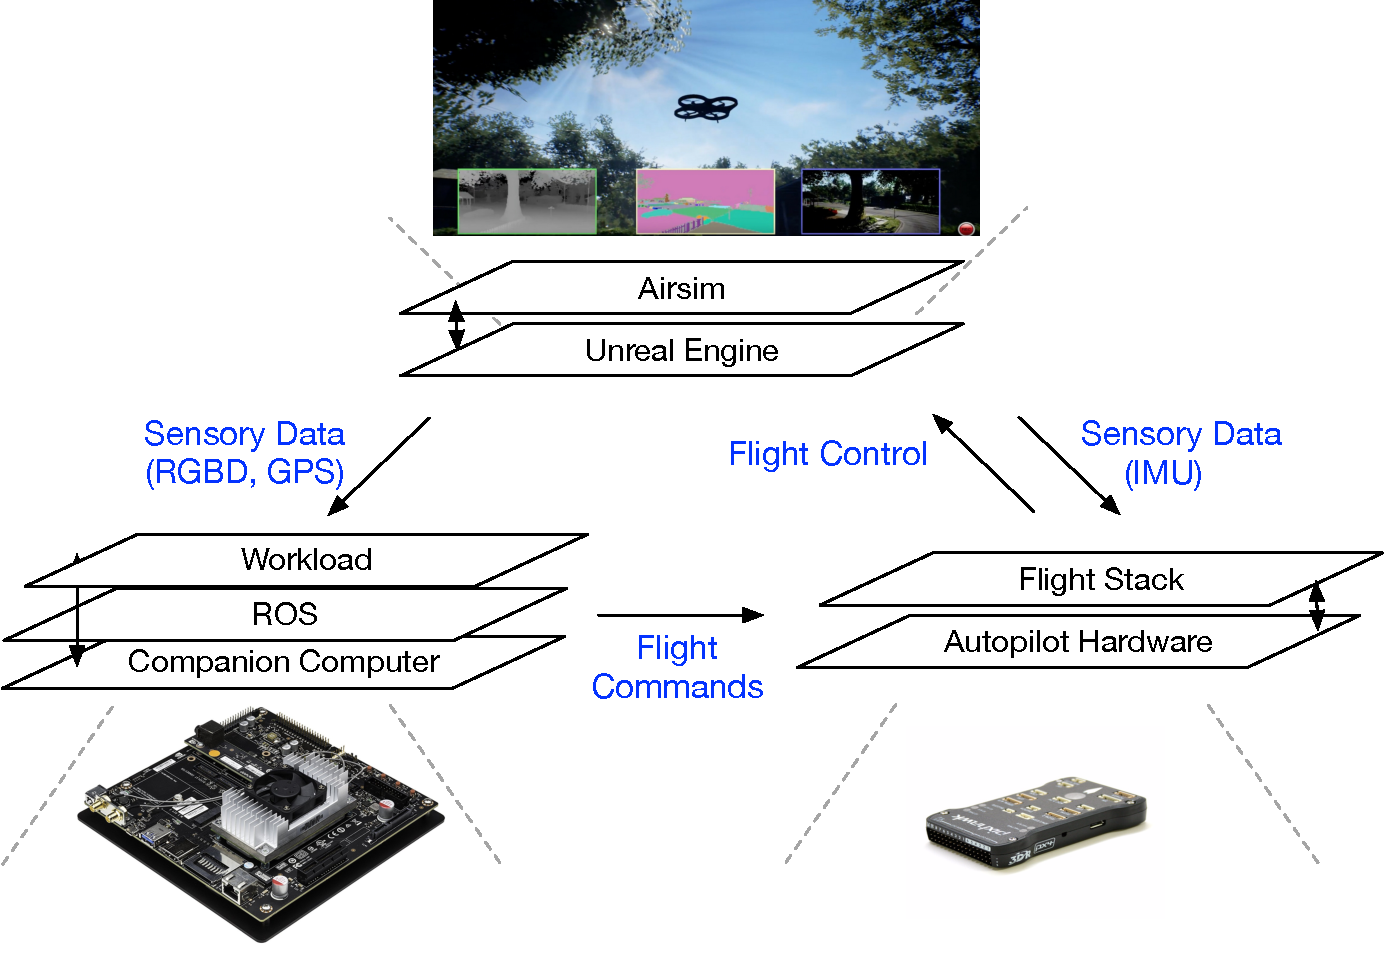
\includegraphics[trim= 10 10 10 10, clip, width=0.75\columnwidth]{figs/end-to-end-simulation}
\caption{Architectural overview of our closed-loop simulation. 
%\red{change airsim to UNREAL + Airsim: possibly annotate them with env and MAV (maybe even sensors/actuators)}}
}
\label{fig:end-to-end}
\end{figure}

\paragraph{Environments, Sensors and Actuators:} Environments, sensors and actuators are simulated with the help of a game engine called Unreal~\cite{GameEngi70:online}. With a physics engine at its heart, it ``provides the ability to perform accurate collision detection as well as simulate physical interactions between objects within the world''~\cite{PhysicsS8:online}. Unreal provides a rich set of environments such as mountains, jungles, urban setups, etc. to simulate.

To capture a MAV's dynamics and kinematics through its actuators' behavior and its sensory modules, we used AirSim, an open-source Unreal based plug-in from Microsoft~\cite{Airsim:online}. We limit our sensors and actuators to the ones realistically deployable by MAVs, such as \mbox{RGB-D} cameras and IMUs. Unreal and Airsim run on a powerful computer (host) capable of physical simulation and rendering. Our setup uses an Intel Core i7 CPU and a high-end NVIDIA GTX 1080 Ti GPU.  

\paragraph{Flight Controller:} AirSim supports various flight controllers that can be either hardware-in-the-loop or completely software-simulated. For our experiments, we chose the default software-simulated flight controller provided by AirSim. However, AirSim also supports other FCs, such as the Pixhawk~\cite{Pixhawk:online}, shown in black in \Fig{fig:end-to-end} which runs the PX4~\cite{PX4Archi7:online} software stack. AirSim supports any FC which can communicate using MAVLINK, a widely used micro aerial vehicle message marshaling library~\cite{mavlinkm68:online}. %MAVLINK is supported as the communication protocol by an extensive number of autopilot systems.
%\red{we should somehow here or later mention that we actually are using the airsim's simple FC instead of pixhawk}


\paragraph{Companion Computer:} We used an NVIDIA Jetson TX2~\cite{TX2}, a high-end embedded platform from Nvidia with 256 Pacal CUDA cores GPU and a Quad ARM CPU; however, the flexibility of our setup allows for swapping this embedded board with others such as x86 based Intel Joule~\cite{joule:online}. TX2 communicates with Airsim and also FC via Ethernet.

\paragraph{ROS:} Our setup uses the popular Robot Operating System (ROS) for various purposes such as low-level device control and inter-process communication~\cite{ROSorgPo80:online}.
Robotic applications typically consist of many concurrently-running processes that are known as ``nodes.'' For example one node might be responsible for navigation, another for localizing the agent and a third for object detection. ROS provides peer-to-peer communication between nodes, either through blocking ``service'' calls, or through non-blocking FIFOs (known as the Publisher/Subscriber paradigm). % A Master node registers all other nodes in a table allowing the communication to take place. 

\paragraph{Workloads:} Our workloads runs within the ROS runtime on TX2. They are extensively discussed in \Sec{sec:benchmarks}.

\paragraph{Putting It All Together:} To understand the flow of data, we walk the reader through a simple workload where the MAV is tasked to detect an object and fly toward it. The object (e.g. a person) and its environment (e.g. urban) are modeled in the Unreal Engine. As can be seen in \Fig{fig:end-to-end}, the MAV's sensors (e.g. accelerometer and \mbox{RGB-D} Camera), modeled in Airsim, feed their data to the flight controller (e.g. physics data to PX4) and the companion computer (e.g. visual and depth to TX2) using MAVLink protocol. The kernel (e.g. object detection), running within the ROS runtime environment on the companion computer, is continuously invoked until the object is detected. Once so, flight commands (e.g. move forward) are sent back to flight controller, where they get converted to a low level rotor instruction stream flying the MAV closer to the person. 

\subsection{Energy Simulation and Battery Model}
\label{sec:energy}

We extended the AirSim simulation environment with an energy and a battery model. Our energy model is a function of the velocity and acceleration of the MAV~\cite{energyaware}. The higher the velocity or acceleration, the higher the amount of energy consumption. Velocity and acceleration values are sampled continuously, their associated power calculated and integrated for capturing the total energy consumed by the agent.

\newcommand{\norm}[1]{\left\lVert#1\right\rVert}

We used a parametric power estimation model proposed in \cite{3DR-energy-model}. The formula for estimating power $P$ is described below:%
\begin{equation}
\begin{aligned}
P = \begin{bmatrix}
		\beta_{1} \\
		\beta_{2} \\
		\beta_{3}
	\end{bmatrix}^{T}
    \begin{bmatrix}
		\norm{\vec{v}_{xy}} \\
		\norm{\vec{a}_{xy}} \\
		\norm{\vec{v}_{xy}}\norm{\vec{a}_{xy}}
	\end{bmatrix}
    +
    \begin{bmatrix}
		\beta_{4} \\
		\beta_{5} \\
		\beta_{6}
	\end{bmatrix}^{T}
    \begin{bmatrix}
		\norm{\vec{v}_{z}} \\
		\norm{\vec{a}_{z}} \\
		\norm{\vec{v}_{z}}\norm{\vec{a}_{z}}
	\end{bmatrix}
    \\
    +
    \begin{bmatrix}
		\beta_{7} \\
		\beta_{8} \\
		\beta_{9}
	\end{bmatrix}^{T}
    \begin{bmatrix}
		m \\
		\vec{v}_{xy} \cdot \vec{w}_{xy} \\
		1
	\end{bmatrix}
\end{aligned}
\label{eqn:power}
\end{equation}

In the Equation~\ref{eqn:power}, $\beta_{1}$, ..., $\beta_{9}$ are constant coefficients determined based on the simulated drone. $\vec{v}_{xy}$ and $\vec{a}_{xy}$ are the horizontal speed and acceleration vectors whereas  $\vec{v}_{z}$ and $\vec{a}_{z}$ are the corresponding vertical values. $m$ is the mass and $\vec{w}_{xy}$  is the vector of wind movement. 

We have a battery model that implements a coulomb counter approach~\cite{coulomb-counter}. The simulator calculates how many coulombs (product of current and time) have passed  through the drone's battery over every cycle. This is done by calculating the power and the voltage associated with the battery. The real-time voltage is modeled as a function of the percentage of the remaining coulomb in the battery as described in ~\cite{battery-model}.

\subsection{Simulation Knobs and Extensions}
\label{sec:knobs}

With the help of Unreal and AirSim, our setup exposes a wide set of knobs. Such knobs enable the study of agents with different characteristics targeted for a range of workloads and conditions. For different environments, the Unreal market provides a set of maps free or ready for purchase. Furthermore, by using Unreal programming, we introduce new environmental knobs, such as (static) obstacle density, (dynamic) obstacle speed, and so on. In addition, Unreal and AirSim allow for the MAV and its sensors to be customized. For example, the cameras' resolution, their type, number and positions all can be tuned according to the workloads' need.   

Our simulation environment can be extended. For the compute on the edge, the TX2 can be replaced with other embedded systems or even micro-architectural simulators, such as gem5. Sensors and actuators can also be extended, and various noise models can be introduced allowing for reliability studies. 

\subsection{Simulation Fidelity and Limitations}
\label{sec:accuracy}

The fidelity of our end-to-end simulation platform is subject to different sources of error, as it is with any simulation setup. The major obstacle is the \textit{reality gap}---i.e., the difference between the simulated experience and the real world. This has always posed a challenge for robotic systems. The discrepancy results in difficulties where the system developed via simulation does not function identically in the real world. 

To address the reality gap, we iterate upon our simulation components and discuss their fidelity and limitations. Specifically, this involves (1) simulating the environment, (2) modeling the drone's sensors and flight mechanics, and last but not least (3) evaluating the compute subsystem itself.

First, the Unreal engine provides a high fidelity environment. By providing a rich toolset for lighting, shading, and rendering, photo-realistic virtual worlds can be created. In prior work~\cite{unrealcv}, authors examine photorealism by running a Faster-RCNN model trained on PASCAL in an Unreal generated map. The authors show that object detection precision can vary between 1 and 0.1 depending on the elevation and the angle of the camera. Also, since Unreal is open-sourced, we pro grammatically emulate a range of real-world scenarios. For example, we can set the number of static obstacles and vary the speed of the dynamic ones to fit the use case.   

Second, AirSim provides high fidelity models for the MAV, its sensors and actuators. Embedding these models into the environment in a real-time fashion, it deploys a physics engine running with 1000~\si{\hertz}.  As the authors discuss in~\cite{Airsim_paper}, the high precision associated with the sensors, actuators and their MAV model, allows them to simulate a Flamewheel quadrotor frame equipped with a Pixhawk~v2 with little error. 

Flying a square-shaped trajectory with sides of length 5~\si{\meter} and a circle with a radius of 10~\si{\meter},  AirSim achieves  0.65~\si{\meter} and 1.47~\si{\meter} error, respectively. Although they achieve high precision, the sensor models, such as the ``camera lens models,'' ``degradation of GPS signal due to obstacles,'' ``oddities in camera,'' etc. can benefit from further improvements. %\red{somewhere we should mention that we extended airsim to use DJI Matrice}

Third, as for the compute subsystem itself, our hardware has high fidelity since we use off-the-shelf embedded platforms for both the companion computer and the flight controller. As for the software, it is crucial to note ROS is widely used and adopted as the \textit{de facto} OS in the robotics research community.

%The details of the simulation environment components' precisions resulting in the aforementioned error is further discussed in~\cite{Airsim_paper}.

%\subsection{Simulation Limitations}
%\label{sec:limits}

%\paragraph{Network Bottleneck:} As was previously mentioned, our companion computer and Airsim are connected through Ethernet. Hence, transferring multiple high resolution images can be throttled by the cable's bandwidth. 

\begin{comment}
Using such data, one can define  various metrics for the applications of interest. For example, using time to delivery over the amount of energy spent, one can define an efficiency metric for a package delivery application. Metrics are extensively discussed in the section \ref{MAVBench characterization}.
\end{comment}
\begin{comment}
\begin{figure*}[h]
\centering
\includegraphics[width=.3\linewidth]{figs/blank}
\includegraphics[width=.3\linewidth]{figs/blank}
\includegraphics[width=.3\linewidth]{figs/blank}
\caption{Show a picture of what AirSim is doing and what the "MAV" is seeing.}
\label{fig:end-to-end}
\end{figure*}
\end{comment}

\begin{comment}

\subsection{Workloads} \label{ssec:benchmarks}

\red{here we explain the workloads we are using for our study, going into the details of each and perhaps even explaining what computational kernels they are exercising. the table of the workloads should discuss the internal details of th apps.}

Our workloads are organized into a full benchmark suite that tests a MAV's ability to perform the tasks required for popular MAV applications today as well as MAV applications that are expected to become significant in the near-future.

Our benchmark suite is divided into two categories: a set of micro-benchmarks that test narrow MAV capabilities and a set of macro-benchmarks that test full MAV applications.

\subsubsection{Micro-benchmarks} \label{sssec:micro}

Our micro-benchmarks test a MAV's ability to execute tasks that would be part of a full MAV application, such as computational kernels or simple flight maneuvers. The micro-benchmarks themselves, however, do not represent complete MAV applications.

The micro-benchmarks primarily stress a MAV's computer vision, SLAM, and pathfinding capabilities. A few of the micro-benchmarks do not test any computational capabilities at all, but are instead meant to characterize a MAV's power consumption during flight. Our micro-benchmarks are listed in full in Table~\ref{tab:micro}.




\subsubsection{Macro-benchmarks} \label{sssec:macro}

Our macro-benchmarks, described in Table~\ref{tab:macro} are complete MAV applications that characterize a MAV's performance and power consumption when performing typical MAV applications. The macro-benchmarks are made up the smaller kernels that are tested by the micro-benchmarks described in Sec.~\ref{sssec:micro}.

\begin{table*}[h!]
\begin{tabular*}{\textwidth}{l@{\extracolsep{\fill}}lllll}
\hline
Benchmark & Use Case & Kernel(s)\\\hline
\texttt{outdoor\_track} & Target tracking (sports photography) & Computer vision; object detection \\
\texttt{indoor\_track} & Target tracking (indoors) & Computer vision; object detection \\
\texttt{deliver} & Package delivery & Pathfinding; SLAM; computer vision \\
\texttt{search} & Search and rescue & Computer vision; object detection; SLAM \\
\texttt{survey} & Land surveying & \fxnote{nothing really} \\
\texttt{map} & Mapping a building & Computer vision; image stitching \\
\texttt{data\_coverage} & Wireless data coverage & \fxnote{?} \\
\texttt{driving} & Autonomous navigation & Machine learning \\
\texttt{take\_picture} & Go to target address, take picture, and return & Path planning \\
\hline
\end{tabular*}
\caption{Macro-benchmarks.}
\label{tab:macro}
\end{table*}

\subsection{Platforms} \label{ssec:MAVs}

\red{here we provide the specific platforms we have evaluated, and for the most part these will be the architectural capabilities of the compute boards that corresponds to our different MAV platforms.}

% Description of our MAV platforms, including a table giving details on each one's weight, flight controller, etc.

We characterize a variety of MAV processors and MAV platforms, both physical and simulated, using our benchmark suite. Our power characterizations are based primarily upon our physical MAVs, described in Table~\ref{tab:MAV-platforms}. Our performance characterizations are primarily based upon workloads run on a simulated MAV known as Microsoft AirSim~\cite{}, rather than on physical MAV platforms.

\paragraph{Processors} We run our computational workloads on a variety of embedded processors, described in Table~\ref{}, that are targeted towards MAVs and robotics applications. These range from state-of-the-art embedded systems with powerful CPUs and hundreds of GPU cores all the way to smartphone-level processors such as the i.MX6 with much lower performance capabilities.

\begin{table*}[t!]
\centering
\caption{Companion computer characteristics.}
\label{tab:cc-platforms}
\begin{tabular}{ l | c c c c c }
 \hline \noalign{\vskip 0.5mm}
 & Intel Aero & Jetson TX1 & Intel Joule & i.MX6 Solo & ODroid  \\
 \hline \noalign{\vskip 0.5mm}
 % SOC    	& Intel Atom 7-Z8750 & \\
 CPU    	& Intel Atom 7-Z8750 & ARM Cortex-A57 & Intel Atom T5700 & ARM Cortex A9 \\
\ \ Frequency	& 1.60 GHz & \fxnote{Unpublished} & 1.7 GHz & 1 GHz \\
\ \ L1 \$ (I/D) & 226 KiB & 80 KB & \fxnote{Unknown}  & 64 KB \\
\ \ L2 \$ (I/D) & 2 MiB & 2 MB  & 2x2 MB & 512 KB \\
\ \ Cores 	& 4 & 4 & 4 & 1 \\
 GPU    	& Intel HD Graphics 405 & 256-core Maxwell GPU & Intel HD Graphics & Two integrated 3D and 2D GPUs\\
 RAM    	& 4 GB LPDDR3 & 4 GB LPDDR4 & 4 GB LPDDR4 & 512 MB \\
 OS     	& Yocto 2.1 (Linux 4.4.3) & Ubuntu 16.04 & Ubuntu 16.04 & 3DR Poky (based on Yocto) \\
 \hline
\end{tabular}
\end{table*}

\paragraph{Physical MAVs} We characterized the power consumption of MAVs ranging from X to Y lbs in weight. We investigated MAVs of different weights because a MAV's weight strongly affects its power consumption and is also correlated to its maximum payload which determines the weight of the components that can be placed upon it. 

% \paragraph{Microsoft AirSim} A simulated MAV with realistic video data. The setup is illustrated in Fig.~\ref{fig:end-to-end}.

\paragraph{Microsoft AirSim} AirSim is an HIL simulator of a micro-aerial vehicle that was developed to allow machine learning applications to easily and safely generate training data for their MAVs. AirSim runs on the Unreal engine and is thus capable of generating realistic video data for our MAV applications. Thus, AirSim allow us to develop realistic environments for our macro-benchmarks so that our characterizations can be easily run on MAV processors in a safe and repeatable fashion. The interfacing between our workloads, MAV processors, and AirSim itself in illustrated in Fig.~\ref{fig:end-to-end}.

\end{comment}